% Cross-modal feature ablation in LLaVA-v1.5-7B
% ============================================================
% Draft 2 -- condensed to a 5-page main body; supporting material in appendices.
% ============================================================
\documentclass[11pt,a4paper]{article}

\usepackage[T1]{fontenc}
\usepackage{lmodern}
\usepackage[margin=2.5cm]{geometry}
\usepackage{amsmath,amssymb}
\usepackage{graphicx}
\usepackage{booktabs}
\usepackage{multirow}
\usepackage{array}
\usepackage{hyperref}
\usepackage{xcolor}
\usepackage{microtype}
\usepackage{parskip}
\usepackage[round]{natbib}

\hypersetup{colorlinks=true, linkcolor=blue!60!black,
            citecolor=green!50!black, urlcolor=blue!60!black}

\graphicspath{{paper_figures/}{figures/}}

\title{\textbf{Calibrating Sparse Autoencoder Ablation Against Attention Knockout in a Vision-Language Model}}
\author{Ron Kremer}
\date{August 2026 --- draft}

\begin{document}
\maketitle

% ============================================================
\begin{abstract}
\noindent
Sparse autoencoders (SAEs) have been used in mechanistic interpretability and
model steering research to make causal claims about the locality of model
behavior: replace the outputs of a layer with a reconstruction, ablate a set
of latent SAE features, observe a behavioral change, and conclude that those
features carry the mechanism that controls the target behavior. In this study,
we use SAEs to better understand the mechanism of cross-modal information
transfer (CMIT), the process by which the model combines visual and textual information, in Vision-Language Models. 
We find that CMIT is distributed across a narrow range of layers, and that feature ablation at a single layer
recovers only a fraction of the effect achieved by a distributed intervention.
In a decoder-only VLM, attention is the only operation that moves information
between token positions, so attention knockout from question positions to
image positions removes cross-modal transfer at a layer, and yields an
estimate of the maximum effect available at that layer. Measured against this
estimate, single-layer SAE ablation saturates: at the layer with the strongest
transfer, a twentyfold increase in the size of the ablated feature set (top-k
from 40 to 800) yields little change, while its perturbation of the residual
stream more than triples. Ablating the same number of features spread across
five layers recovers three times the effect at half the perturbation.
Compensation by downstream layers re-reading the image, the leading account of
such a ceiling, is rejected on four tests. Where a feature budget is allocated
therefore constrains the measured effect more than its size, and the saturation 
observed at a single layer is not evidence that the selected features account 
for the mechanism.
\end{abstract}


% ============================================================
\section{Introduction}

Sparse autoencoders (SAEs) decompose transformer activations into an
overcomplete basis of sparse, putatively interpretable directions
\citep{bricken2023monosemanticity,templeton2024scaling}, and are increasingly
used to support causal claims about mechanism. The evidence offered is typically
an ablation of the selected features against random features of equal size. That
comparison establishes that the selection is better than chance. It does not
establish how much of the mechanism the features account for, nor whether a
larger or differently allocated set would account for more --- and without an
independent estimate of the total effect, a flat response to added features is
indistinguishable from having captured everything available.

Vision-language models make the question tractable. In a decoder-only VLM with
image tokens prepended to the text sequence, visual information reaches the
prediction through attention from text positions to image positions
\citep{zhang2024crossmodal,neo2025towards}, which fixes a site, a set of
positions, and an intervention that severs the pathway without reference to any
dictionary. Attention knockout at a layer thus supplies a behavioural scale
against which feature ablation at the same locus can be read.

We report three results from 47 intervention conditions on a common item set.
Feature ablation at a single layer saturates: a twentyfold increase in budget at
the layer with the strongest cross-modal transfer moves the effect by less than
0.05, while the disturbance inflicted on the residual stream more than triples.
The same budget spread across five layers is 2.90 times as effective at roughly
half the disturbance, so the binding constraint is allocation rather than size
or force. And the leading explanation for the ceiling --- that downstream layers
re-read the image and restore what was removed --- fails four tests.

\paragraph{Related work.} Attention knockout localises cross-modal transfer by
layer and by position in decoder-only VLMs \citep{zhang2024crossmodal,neo2025towards,jiang2025devils},
which makes those findings layer-resolved but not content-resolved. Dictionary
methods supply content, and their application to VLMs is recent:
\citet{yang2026monet} report many near-duplicate visual features recurring
across adjacent layers and call for cross-layer analysis designs, while
\citet{lindsey2025circuittracing} note that transcoders sidestep the
layer-boundary problem per-layer SAEs face. We rank features by gradient-based
causal attribution following \citet{marks2024sparsefeaturecircuits}. The
hypothesis we test and reject is the multimodal analogue of self-repair
\citep{mcgrath2023hydra,rushing2024selfrepair}: because image tokens survive a
question-position ablation unmodified, downstream layers could re-read the
source directly rather than reconstructing it.

% ============================================================
\section{Setup}

\paragraph{Model and task.} All experiments use LLaVA-v1.5-7B
\citep{liu2023llava}: CLIP ViT-L/14-336px, a two-layer projector, and a 32-layer
Vicuna-1.5-7B decoder ($d_{\text{model}} = 4096$), with images entering as 576
prepended patch tokens. CLEVR-Lite is a synthetic forced-choice VQA set built
for this study in the style of CLEVR \citep{johnson2017clevr}: 50{,}000 rendered
scenes, three question templates, and a closed vocabulary of six colours and
three shapes, each question paired with one true answer and one distractor drawn
from the remaining members of the relevant set. It replaces GQA ChooseAttr
\citep{hudson2019gqa}, which presents both candidates in the prompt and so
admits a language-side route to the answer that survives complete removal of
visual information. Effects are the mean drop in the logit margin
$\Delta = \log P(a_{\text{true}}) - \log P(a_{\text{false}})$ relative to an
unmodified pass. The margin is preferred to accuracy, which is a thresholded
function of it and insensitive to sub-threshold change. Two accuracy notions
appear below and are not interchangeable: forced-choice accuracy, the fraction
of items with a positive margin, and generation accuracy, the fraction whose
greedily decoded answer matches the target string. The latter is depressed by
truncation of otherwise correct answers and is reported only as a secondary,
conservative check.

\paragraph{Site and positions.} One SAE is trained per layer on the attention
output (\texttt{attn\_out}) at question-token positions, with 32{,}768 features
and $\ell_1$ coefficient $5\times10^{-4}$ (Appendix~A). Reading attention output
rather than the residual stream places ablation and knockout at the same locus,
so their comparison concerns what is removed rather than where. Question
positions are forced by the design: Image$\rightarrow$Question knockout leaves
image-token residual streams unchanged by construction, so any measurement at
image positions is null whatever the model is doing. These dictionaries are not
sparse in the usual sense --- mean $L_0$ is 1{,}128 to 1{,}587 of 32{,}768, a
density of 3.4--4.8\% --- so a 200-feature ablation removes on the order of 15\%
of the active features at a site.

\paragraph{Feature selection and ablation.} Features are ranked by
$s_i = |\partial \Delta / \partial z_i| \cdot |z_i|$, computed with the
autoencoder inserted differentiably into the forward pass, and the top $k = 200$
per layer are selected unless stated otherwise. A fixed budget across layers is
what makes the concentrated-against-spread contrast a comparison of allocation;
the value is not otherwise load-bearing. Selected features are removed in
\texttt{replace} mode: the activation is encoded, the selected coefficients are
zeroed, and the decoded reconstruction replaces the original for the rest of the
pass. This admits reconstruction error deliberately, so that a zero-feature
intervention exposes it rather than being a no-op; the error is small, with
replace-mode passthrough across five stacked hooks giving $+0.00109$ against a
0.02 threshold. Multi-layer conditions install one hook per layer, each with
its own dictionary and feature set. An
earlier correlational selection metric, the ratio of mean activation on
correctly against incorrectly answered items, fails in this regime and is
reported in Appendix~B.

\paragraph{Evaluation and statistics.} Every condition is evaluated on the same
256 CLEVR-Lite validation questions, verified identical by SHA-1 of the ordered
identifier list, so all comparisons are paired; the unmodified model attains a
mean margin of 2.739, a forced-choice accuracy of 0.914 and a generation
accuracy of 0.648 on this set. Random-feature
controls are matched on mean activation, since unmatched controls conflate
feature identity with perturbation magnitude (Appendix~C). Significance uses the
Wilcoxon signed-rank test and, for the spread-against-concentrated contrast, a
paired bootstrap over questions (20{,}000 resamples). Alongside every effect we
report the mean relative perturbation of the residual stream, which separates an
effect from the force used to produce it.

% ============================================================
\section{Results}

\subsection{The analysis span}

Figure~\ref{fig:landscape} reports the margin drop from blocking cross-modal
attention at each of the 32 decoder layers, over 7{,}084 validation questions.
Image$\rightarrow$Last is the weaker route wherever transfer is substantial: its
largest effect at any layer (0.084, layer 0) is smaller than that of the
fifth-ranked Image$\rightarrow$Question layer, against 0.457 for
Image$\rightarrow$Question at the same layer. Question tokens rather than the
prediction position are therefore the conduit. Five layers separate from the rest: layer 0
($\Delta = 0.457$), 11 (0.427), 14 (0.398), 10 (0.268) and 12 (0.245), against
0.104 for the sixth-ranked layer.

Layers 10--14 were adopted as the analysis span, fixed from this sweep before
any ablation was run. Layer 13 is retained despite an \emph{inhibitory} knockout
effect ($\Delta = -0.048$), since excluding a layer for an unexpected sign would
select the span on the outcome; its exclusion is reported as a sensitivity
analysis instead. Layer 0 is excluded for a reason specific to the instrument:
its dictionary is 74.2\% dead against 0.06--0.4\% at layers 10--14, so ablation
there would measure one dictionary's pathology. The strongest site of
cross-modal transfer is therefore not addressable by the method examined here.

\begin{figure}[t]
  \centering
  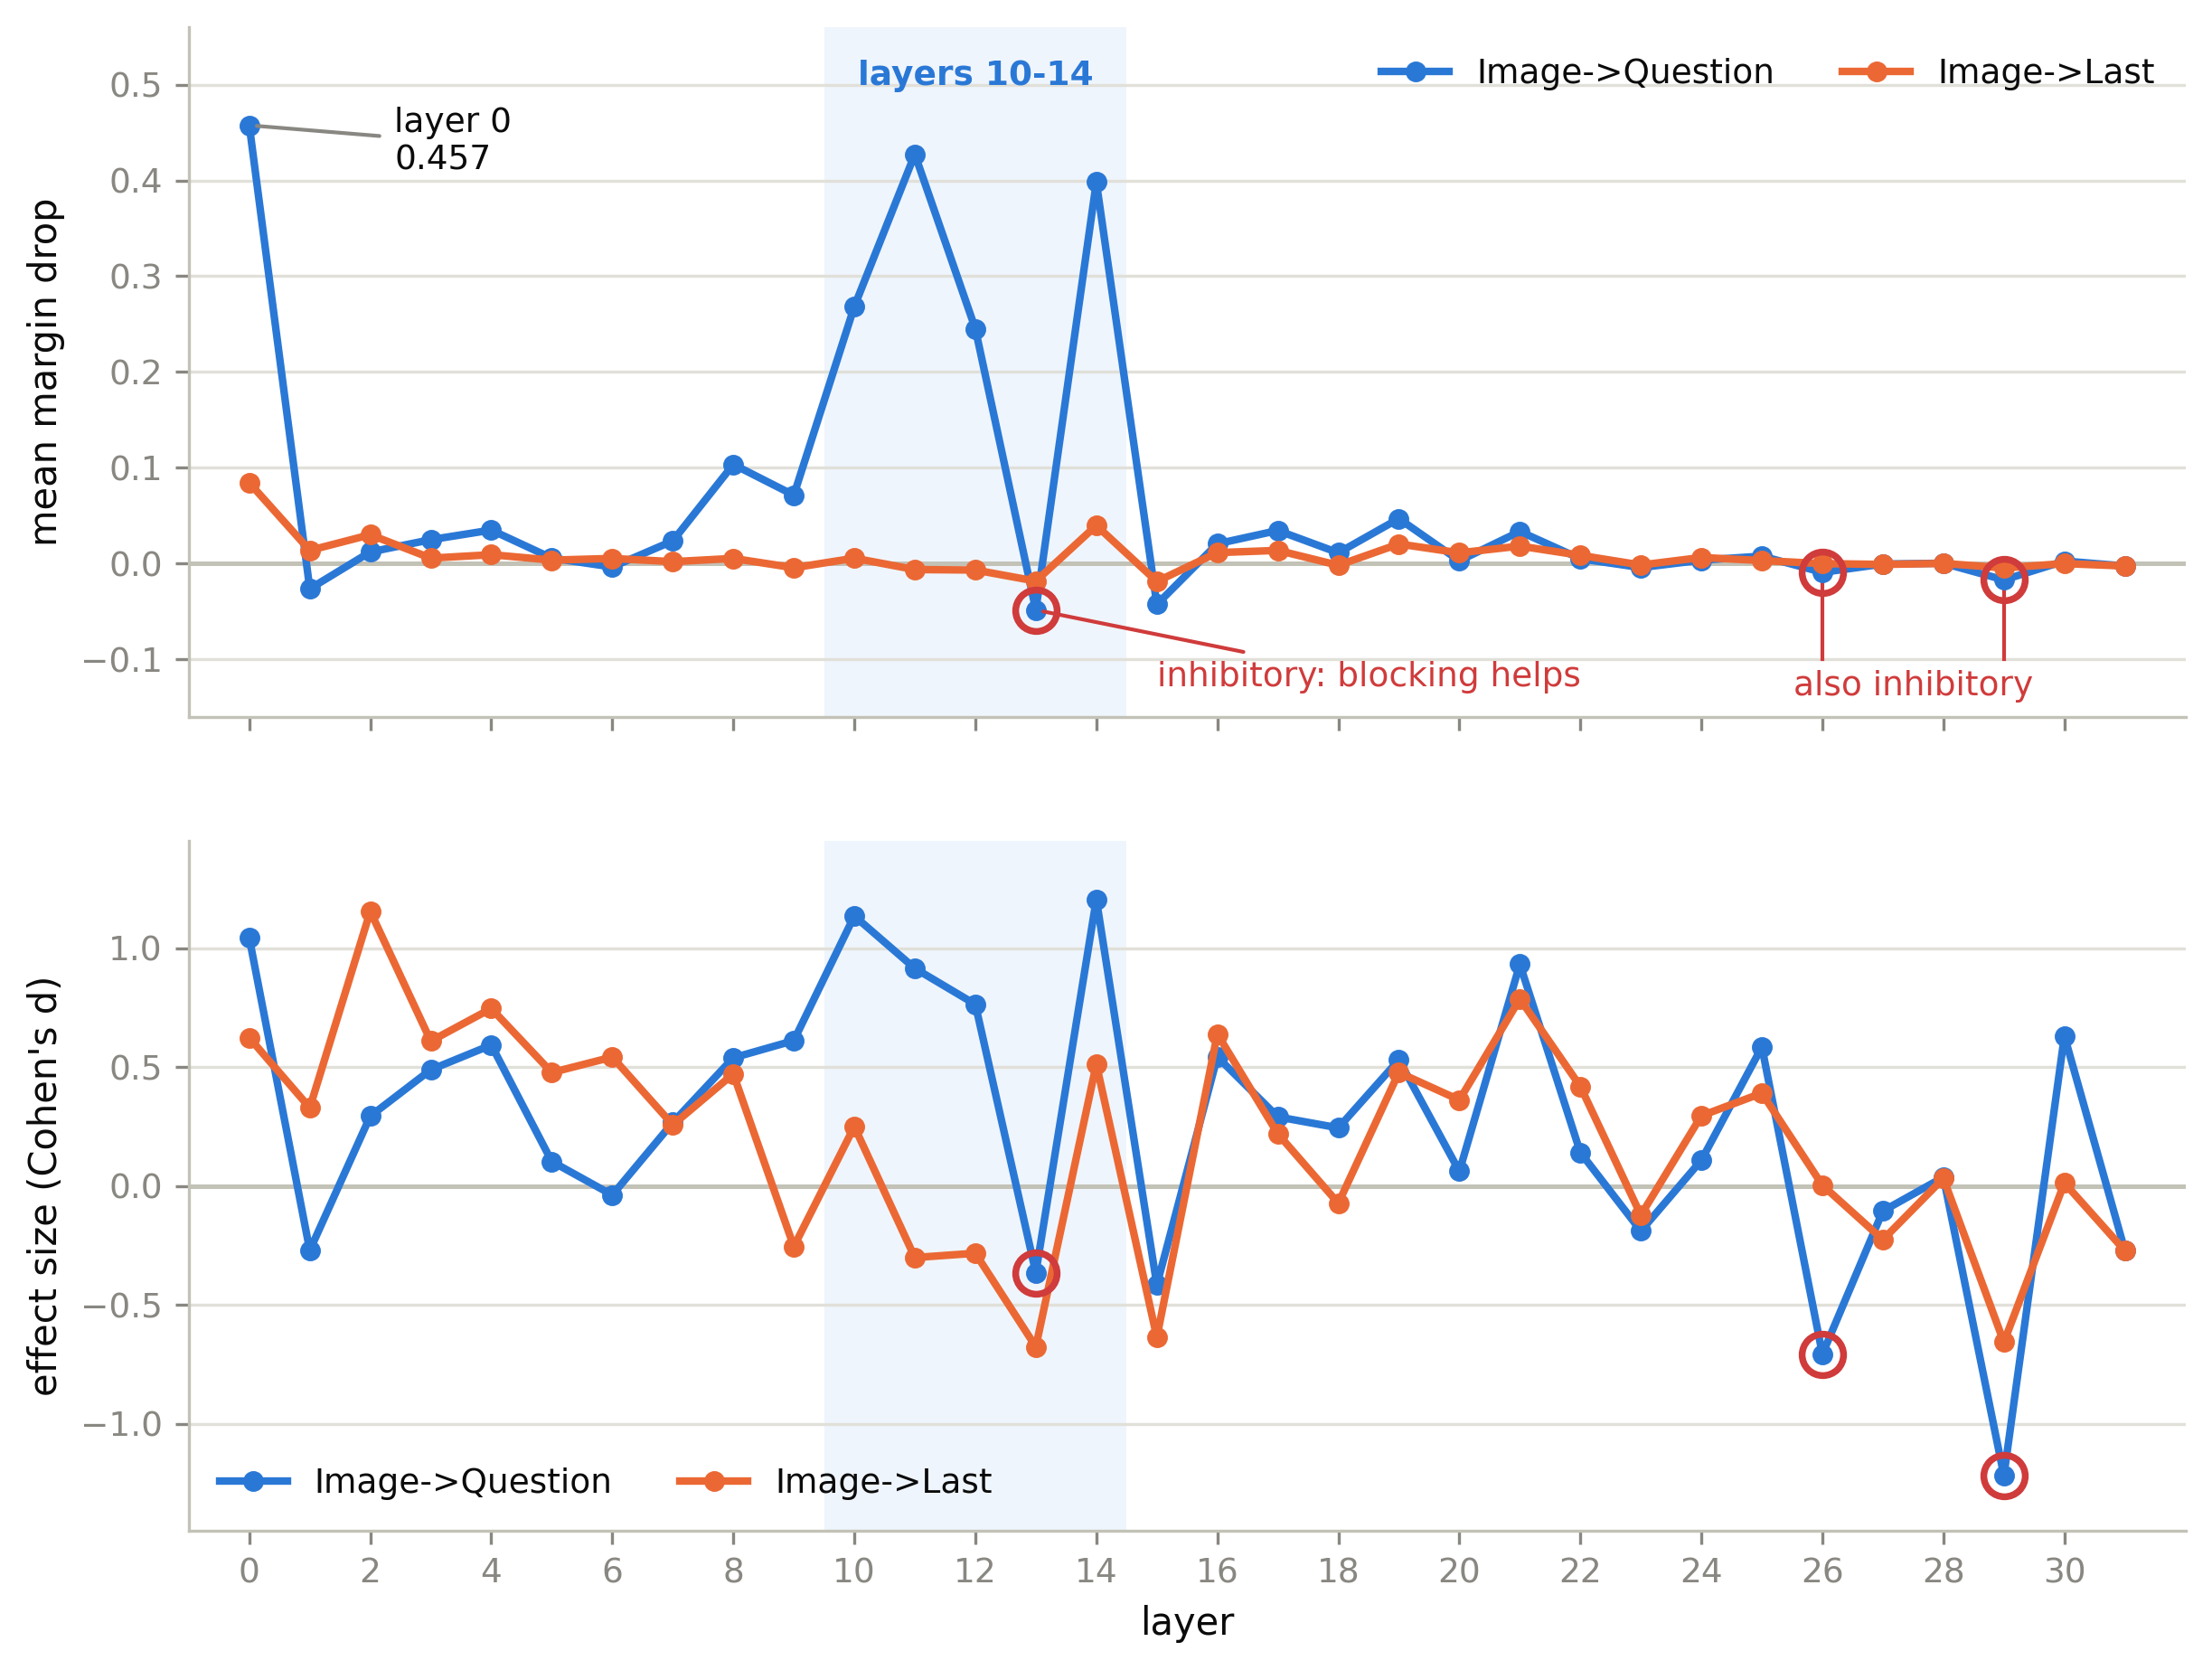
\includegraphics[width=\textwidth]{fig1_knockout_landscape}
  \caption{\textbf{Attention-knockout landscape.} Mean margin drop (top) and
  Cohen's $d$ (bottom) from blocking Image$\rightarrow$Question (blue) and
  Image$\rightarrow$Last (orange) attention at each decoder layer,
  $n = 7{,}084$. The shaded band marks layers 10--14, selected as the analysis
  span from this sweep before any ablation was run.}
  \label{fig:landscape}
\end{figure}

\subsection{A single layer has a ceiling}

Ablating the top 200 causally scored features at one layer produces margin drops
between 0.122 and 0.243 across the span (Appendix~D).
Table~\ref{tab:budget} varies the budget at layer 11, where cross-modal transfer
is strongest.

\begin{table}[t]
  \centering
  \caption{Margin drop and mean relative residual-stream perturbation for two
  allocations of a feature budget. All conditions: \texttt{replace} mode,
  question positions, $n = 256$.}
  \label{tab:budget}
  \begin{tabular}{lrrr}
    \toprule
    Condition & Features & Margin drop & Rel.\ perturbation \\
    \midrule
    Spread, 40 $\times$ 5 layers & 200 & \textbf{0.6182} & 0.0100 \\
    \midrule
    Concentrated L11, $k=40$  &  40 & 0.1895 & 0.0091 \\
    Concentrated L11, $k=100$ & 100 & 0.1920 & 0.0136 \\
    Concentrated L11, $k=200$ & 200 & 0.2131 & 0.0186 \\
    Concentrated L11, $k=400$ & 400 & 0.2364 & 0.0274 \\
    Concentrated L11, $k=800$ & 800 & 0.1940 & 0.0330 \\
    \bottomrule
  \end{tabular}
\end{table}

A twentyfold increase in budget moves the effect from 0.190 to a maximum of
0.236 and back down to 0.194, a range of less than 0.05, while relative
perturbation rises monotonically from 0.0091 to 0.0330. Both obvious
explanations are excluded by direct measurement: the effect scales neither with
the number of features nor with the disturbance inflicted on the residual
stream. Beyond $k \approx 400$ added features perturb the stream without adding
effect. Whatever bounds single-layer ablation is neither budget nor force.

\subsection{The same budget, distributed, is 2.9 times as effective}

Forty features at each of layers 10--14 produce a margin drop of 0.618 against
0.213 for two hundred features at layer 11 (Table~\ref{tab:budget},
Figure~\ref{fig:budget}). A paired bootstrap over the 256 questions gives a ratio of 2.90 (95\% CI
[2.51, 3.37]) and a difference of 0.405 (95\% CI [0.339, 0.475]); the spread
allocation wins on 77.7\% of individual questions (Wilcoxon $p = 1.1 \times
10^{-25}$, $d_z = 0.732$). Generation accuracy falls from 0.648 to 0.520 under
spreading, against at most 2 points at any concentrated budget.

The result is not an artefact of intervention magnitude, which moves in the
opposite direction: the spread condition attains 2.9 times the effect at 54\%
of the perturbation of the equal-budget concentrated condition, and at less
perturbation than every concentrated condition except $k = 40$. Nor is it an artefact of intervening at five sites rather than one.
Forty random features per layer, matched on activation, give a margin drop of
0.105 at \emph{higher} perturbation than the binding arm (0.0126 against 0.0100)
and no accuracy loss, so multi-site intervention on its own recovers about a
sixth of the effect and the identity of the features supplies the remainder.

\begin{figure}[t]
  \centering
  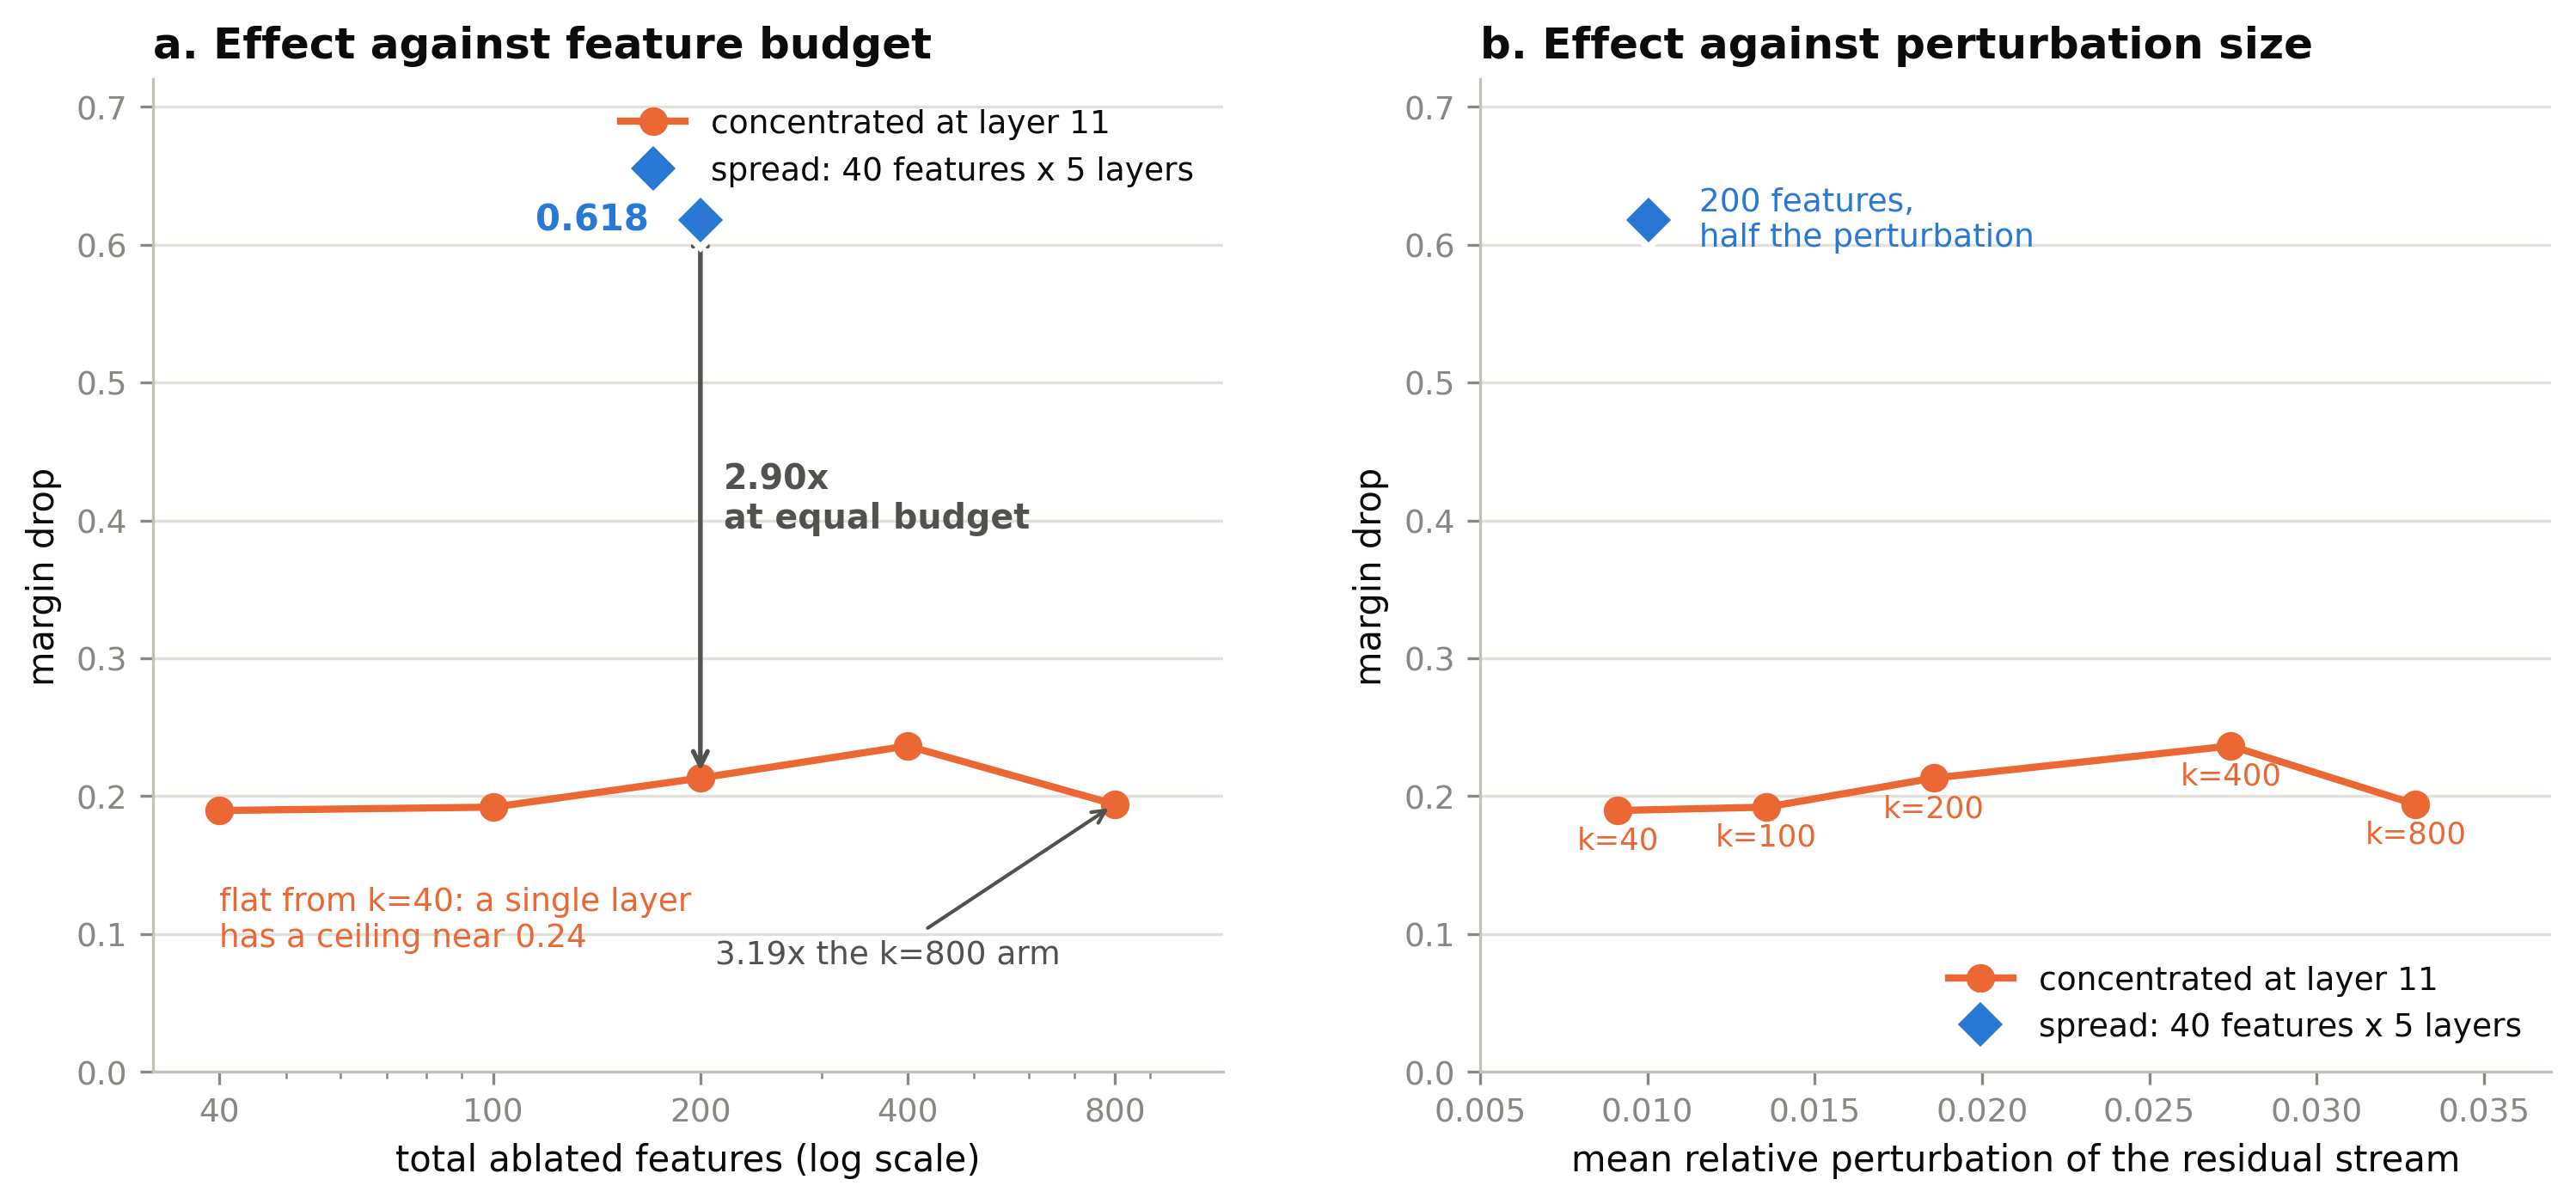
\includegraphics[width=\textwidth]{fig6_budget_distribution}
  \caption{\textbf{Distributing a feature budget outperforms concentrating it.}
  (a) Margin drop against total ablated features for a budget concentrated at
  layer 11 ($k = 40$--$800$) and spread across layers 10--14 (40 per layer).
  (b) The same conditions against mean relative perturbation of the residual
  stream: the spread arm sits up and to the left of the concentrated curve.}
  \label{fig:budget}
\end{figure}

\subsection{Downstream re-reading does not explain the ceiling}

If a single-layer ablation were undone by later layers re-reading the image,
preventing that re-reading should raise the measured effect. It does not. With
Image$\rightarrow$Question attention blocked at every layer downstream of the
anchor, ablation at layer 14 gives a combined effect of 0.599 against an
additive prediction of 0.596, a discrepancy of 0.4\%; at layer 11 the excess is
7.4\%. Three further tests agree (Appendix~D, Figures~\ref{fig:scaling}
and~\ref{fig:rshare}). The ablation arm's superadditivity over
the five-layer span is fully accounted for by the flow's own ($\rho_A = 1.118$
against $\rho_K = 1.146$). Leave-one-out marginal contributions exceed
standalone effects at layers 10, 11 and 12 (ratios 1.14, 1.57, 1.79), the
opposite of the redundancy signature. And spans of equal size but different
composition differ by 0.20 in effect, which a redundancy account has no way to
produce.

Ablation and knockout track each other across the span: they rank the individual
layers in the same order, and over nested spans of one to five layers both grow
linearly at 0.193 and 0.269 per layer, a slope ratio of 0.718. Pooled over those
spans, ablation recovers 72.6\% of the severed pathway (95\% CI
$[69.6, 75.8]$).

That aggregate figure should not be read as a fixed share. Per span, $R = A/K$
runs from 65.1\% to 87.5\%, and no single value lies inside all five intervals
(highest lower bound 81.5\% against lowest upper bound 68.5\%), so the recovered
share genuinely differs between spans. What does not vary is its direction:
$R$ shows no trend with span size (slope $-0.010$ per layer, 95\% CI
$[-0.024, +0.003]$). Compensation by untouched layers predicts the opposite ---
that $R$ rises as the span covers more of the layers doing the compensating ---
so the dispersion is evidence against a redundancy account rather than for one.
It tracks span composition instead, the same way the equal-size spans above do.
The high value at span two is an artefact of the denominator: adding the
inhibitory layer 13 lowers the knockout ceiling from 0.359 to 0.319 while the
ablation rises, so $R$ climbs without any gain in what the features recover.
We read the proportionality
as evidence that ablation follows the pathway knockout severs, and not as a
decomposition of it: knockout removes strictly more than ablation targets, holds
its constraint for the rest of the forward pass where ablation acts once, and at
layer 13 has the opposite sign to the ablation it would otherwise bound.


% ============================================================
\section{Discussion}

Three explanations of the single-layer ceiling remain open, and these
experiments do not separate them. The dictionary at a layer may not contain the
rest of the mechanism, whether because the directions were not learned or
because the mechanism is not expressible in a per-layer basis at all
\citep{yang2026monet,lindsey2025circuittracing}. The selection procedure may saturate before the dictionary does: the gradient
term of the attribution score spans a factor of 2.7 while the activation term
spans seven orders of magnitude, so the ranking exhausts the high-magnitude
features quickly and thereafter buys features that are causally marginal. Or the mechanism may genuinely not be present in full at any
single site, which is the reading the reallocation result supports and the only
one that makes the ceiling a property of the model. Ablating the entire
dictionary at each span would bound the first against the other two, and was not
run.

One confound survives the controls on the distribution result. Five hooks give
the model fewer downstream steps to compensate at each site than one hook does,
so ``the features are distributed'' and ``multi-site interventions are harder to
absorb'' predict the same table. The redundancy tests weigh against the second reading, and the matched-random
spread control bounds it at roughly a sixth of the effect --- though that
control used a single random set, so it admits no interval.

The practical consequence is that a feature ablation at one site reports a
lower bound of unknown tightness: at layer 11 the budget curve is flat while
four fifths of the achievable effect lies elsewhere.

\paragraph{Limitations.} The 256 evaluation questions are the first 256 entries of the validation file
rather than a random draw; the set is verified identical across conditions, so
the paired internal contrasts hold, but generalisation to the validation
distribution is not established. Results come from one model, one synthetic task, one dictionary placement and
one seed per layer, with the strongest transfer layer excluded. And the attribution ranking is dominated by activation magnitude, with the
$|\nabla|$-only against $|z|$-only decomposition unrun.

\paragraph{Availability.} Code, configurations and the per-condition result
summaries backing every number reported here are at
\url{https://github.com/KremerML/cross-modal-information-flow-in-MLLM}. CLEVR-Lite
regenerates deterministically from the committed generator and seed, and each of
the 47 conditions retains its per-question margin drops in the ordering the
paired tests assume, guarded by the SHA-1 of the question list, so those tests
reproduce from a clone without the model.

% ============================================================
\appendix
\section{Configuration}

\begin{table}[h]
  \centering
  \caption{SAE training configuration and reconstruction quality. All layers
  share: 32{,}768 features ($8\times$ expansion over $d_{\text{model}} = 4096$),
  $\ell_1$ coefficient $5 \times 10^{-4}$, learning rate $2 \times 10^{-4}$,
  batch size 256, 10 epochs, float32, seed 42, site \texttt{attn\_out}, question
  positions. Corpus: CLEVR-Lite train split, 186{,}638 questions over 50{,}000
  scenes, 4{,}898{,}438 activation rows.}
  \label{tab:sae}
  \begin{tabular}{lrrrr}
    \toprule
    Layer & Explained var. & Normalised MSE & Mean $L_0$ & Dead fraction \\
    \midrule
    0  & 0.999834 & $1.66 \times 10^{-4}$ & 1416.1 & 0.7419 \\
    10 & 0.998881 & $1.12 \times 10^{-3}$ & 1128.0 & 0.00201 \\
    11 & 0.998513 & $1.49 \times 10^{-3}$ & 1180.1 & 0.00385 \\
    12 & 0.999359 & $6.41 \times 10^{-4}$ & 1587.2 & 0.00061 \\
    13 & 0.998592 & $1.41 \times 10^{-3}$ & 1256.0 & 0.00150 \\
    14 & 0.998695 & $1.30 \times 10^{-3}$ & 1446.5 & 0.00156 \\
    \bottomrule
  \end{tabular}
\end{table}

CLEVR-Lite validation contains 7{,}790 questions; the 256-question evaluation
set is the first 256 entries, spanning 67 scenes. The 32-layer knockout sweep is
evaluated on the 7{,}084 validation items the unmodified model answers
correctly, on which the mean baseline margin is 3.178. In-harness knockouts on
the 256-question set are 0.2665, 0.4268, 0.2135, $-0.0506$ and 0.3593 for layers
10--14, reproducing the sign and ordering of the larger sweep. The 47-condition
sweep ran in 3\,h\,45\,m on an RTX 4090, median binding pass 81.3\,s.

\section{Feature selection: correlational against causal}

The original selection metric ranked features by the ratio of mean activation on
correctly against incorrectly answered items,
$(\bar{z}^{+} + \epsilon)/(\bar{z}^{-} + \epsilon)$ with $\epsilon = 10^{-8}$.
It is numerically unstable in a sparse regime: 176 of the 200 features it
selected at layer 11 have $\bar{z}^{-} = 0$ exactly, so their ranking is set by
$\epsilon$ rather than by any activation difference. The selected features have
mean activation $1.2 \times 10^{-6}$ against a residual-stream norm of
approximately 5.5, and share no members with the attribution-ranked set
(Figure~\ref{fig:ghost}). Eighteen ablation conditions built on this selection
returned null results that would reasonably have been read as evidence about the
model. The failure is diagnosable without a causal reference --- inspecting the
selected features' activation magnitudes against the norm of the stream they are
meant to perturb suffices.

\begin{figure}[h]
  \centering
  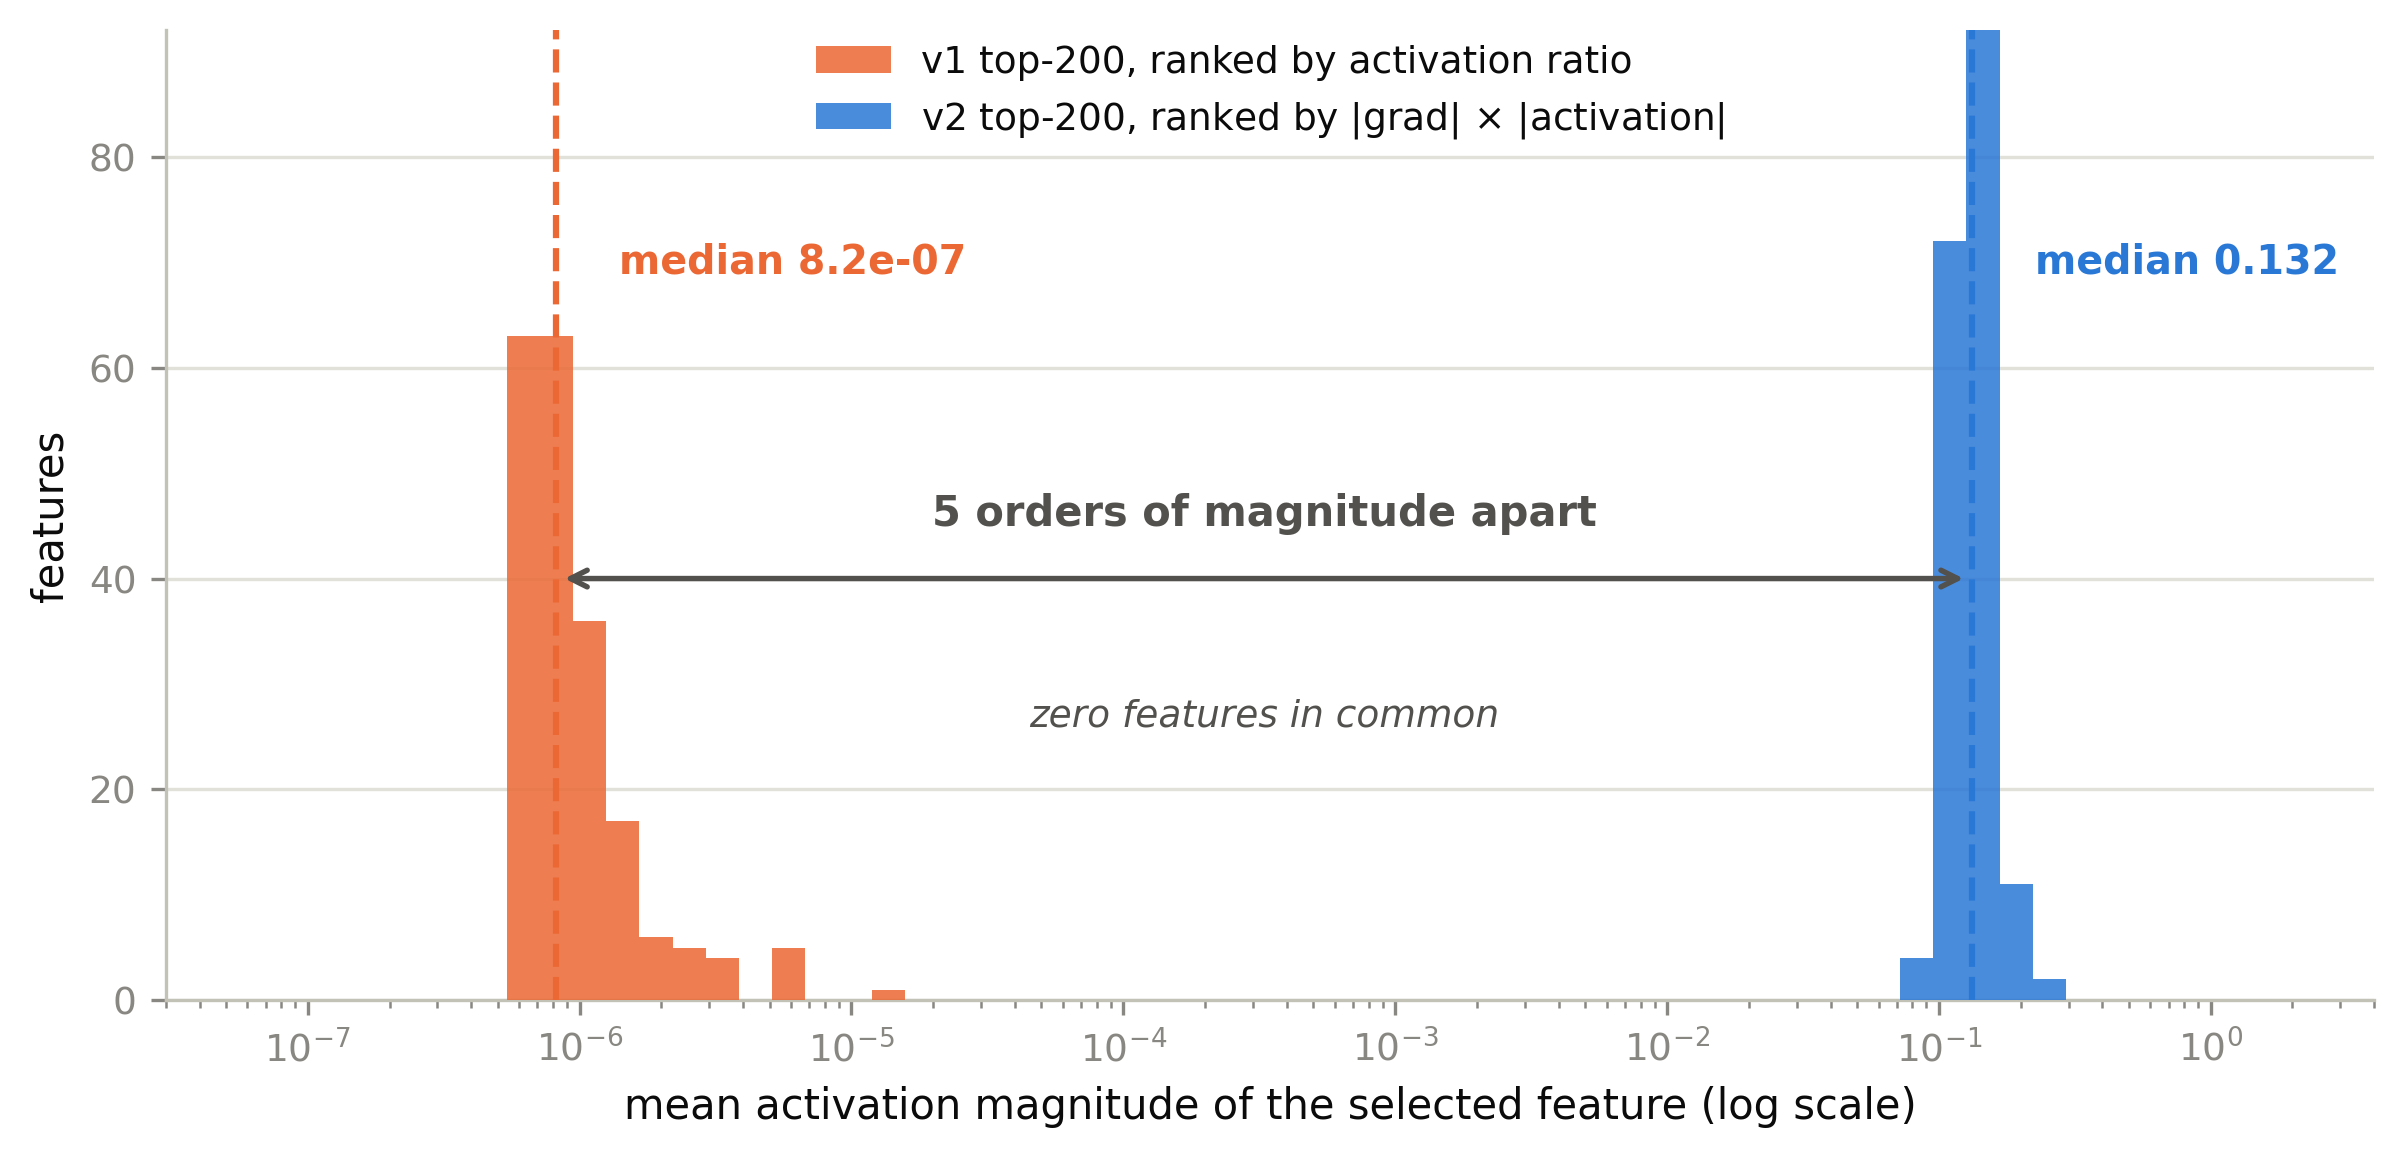
\includegraphics[width=\textwidth]{fig4_v1_ghost_features}
  \caption{Mean activation magnitude of the 200 features selected by the
  correlational ratio against the 200 selected by causal attribution, at layer
  11 of the same dictionary. The two sets are five orders of magnitude apart and
  share no members.}
  \label{fig:ghost}
\end{figure}

\section{Controls and harness validation}

Table~\ref{tab:controls} isolates the effect of the control regime at layer 11,
$k = 200$, holding the intervention fixed. Under matched controls the control
arm perturbs the residual stream \emph{more} than the binding arm while
producing a margin drop near zero; unmatched controls understate the
perturbation and inflate $z$. Two conditions carry 15 control sets --- layer-11
$k{=}200$ ($z = 64$, SE 12) and the joint five-layer span ($z = 111$, SE 21);
the remaining 45 carry one, so no $z$ is reported for them, and control arms
store aggregate summaries rather than per-sample records, so no control
comparison in this paper can be paired or bootstrapped.

\begin{table}[h]
  \centering
  \caption{Control regime at layer 11, $k = 200$. The binding arm is identical
  in both rows (margin drop 0.2131, relative perturbation 0.0186).}
  \label{tab:controls}
  \begin{tabular}{lrrrr}
    \toprule
    Control & Mean & SD & Rel.\ perturbation & $z$ \\
    \midrule
    Uniform            & $-0.0004$ & 0.0026 & $\approx 0.0019$ & 81.6 \\
    Activation-matched & $-0.0217$ & 0.0037 & 0.0225 & 63.5 \\
    \bottomrule
  \end{tabular}
\end{table}

Null interventions behave as expected: no hooks gives exactly 0.0, delta-mode
passthrough across layers 10--14 gives exactly 0.0, and replace-mode passthrough
gives $-0.00037$ to $+0.00109$ across spans of one to five layers, so
reconstruction error does not compound across stacked hooks. Two in-harness
regressions reproduce independently run single-layer values to
$7.7 \times 10^{-6}$ (layer 11) and $8.4 \times 10^{-5}$ (layer 14). Standalone
values for layers 10, 12 and 13 come from earlier runs joined to the sweep by
hash of the ordered question set; they feed $\rho_A$ and the leave-one-out table,
which are therefore cross-run quantities.

\section{Per-layer and per-span results, and redundancy tests}

\begin{table}[h]
  \centering
  \caption{Ablation $A$ and knockout $K$ on the same 256 questions, per layer and
  per span, with paired bootstrap intervals on $R = A/K$ (10{,}000 resamples of
  the question set, applied to both arms together). $R$ is undefined at layer 13,
  whose knockout is inhibitory. Intervals are absent for layers 10 and 12 because
  their ablations predate this harness: the drops are comparable, but there is no
  per-question record to pair against the knockout arm.}
  \label{tab:spans}
  \begin{tabular}{llrrrl}
    \toprule
    & Layer / span & $A$ & $K$ & $R$ & 95\% CI \\
    \midrule
    \multirow{5}{*}{Single}
      & 10 & 0.1514 & 0.2665 & 56.8\% & --- \\
      & 11 & 0.2131 & 0.4268 & 49.9\% & [44.8, 55.3] \\
      & 12 & 0.1670 & 0.2135 & 78.2\% & --- \\
      & 13 & 0.1220 & $-0.0506$ & --- & --- \\
      & 14 & 0.2432 & 0.3593 & 67.7\% & [63.3, 72.2] \\
    \midrule
    \multirow{4}{*}{Nested}
      & \{13,14\}     & 0.2679 & 0.3191 & 83.9\% & [77.9, 90.0] \\
      & \{12,13,14\}  & 0.5007 & 0.5721 & 87.5\% & [81.5, 94.4] \\
      & \{11--14\}    & 0.8302 & 1.2762 & 65.1\% & [61.9, 68.5] \\
      & \{10--14\}    & 1.0028 & 1.3934 & 72.0\% & [68.9, 75.3] \\
    \midrule
    \multirow{2}{*}{Size 3}
      & \{10,11,12\}  & 0.7590 & 1.2975 & 58.5\% & [55.2, 62.1] \\
      & \{10,12,14\}  & 0.5631 & 0.7648 & 73.6\% & [69.9, 77.5] \\
    \midrule
    Sensitivity & \{10,11,12,14\} & 0.9166 & 1.3673 & 67.0\% & [64.0, 70.4] \\
    \bottomrule
  \end{tabular}
\end{table}

\begin{figure}[h]
  \centering
  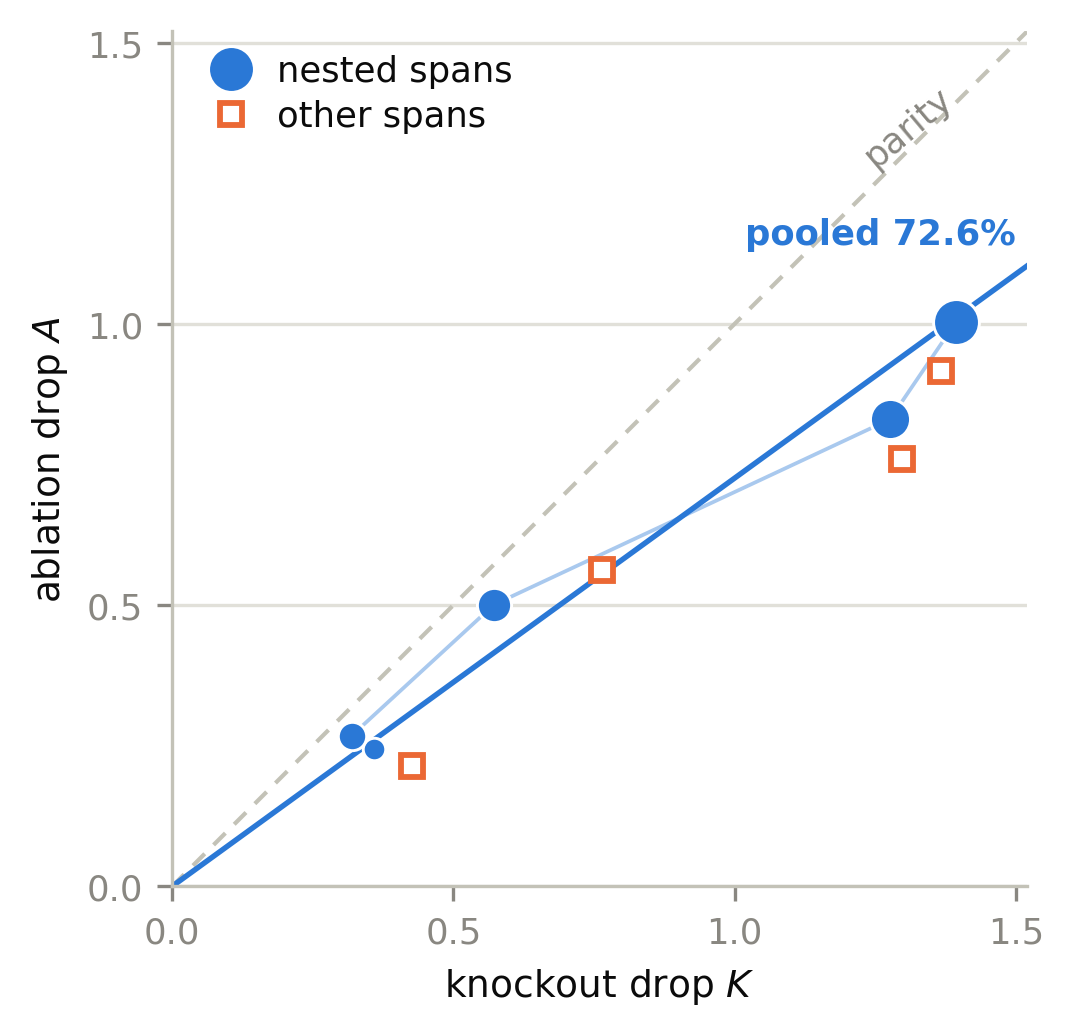
\includegraphics[width=0.58\textwidth]{fig8a_ablation_vs_knockout}
  \caption{\textbf{Ablation scales with the pathway rather than saturating against
  it.} Ablation drop $A$ against knockout drop $K$, one point per condition on the
  same 256 questions, marker area increasing with span size. Filled circles are the
  nested spans grown downward from layer 14, joined in span order; open squares are
  the other compositions (layer 11 alone, the two non-nested three-layer spans, and
  the layer-13 sensitivity span). Every condition falls below parity (dashed) and
  near one line through the origin at the pooled recovery of 72.6\%; in aggregate
  the two curves grow at 0.193 and 0.269 per layer, a slope ratio of 0.718. Marker
  size shows no pattern about that line, which is the absence of a span-size effect
  seen without taking a ratio. The path runs backwards in $K$ between the first two
  nested spans because the inhibitory layer 13 lowers the ceiling.}
  \label{fig:scaling}
\end{figure}

\begin{figure}[h]
  \centering
  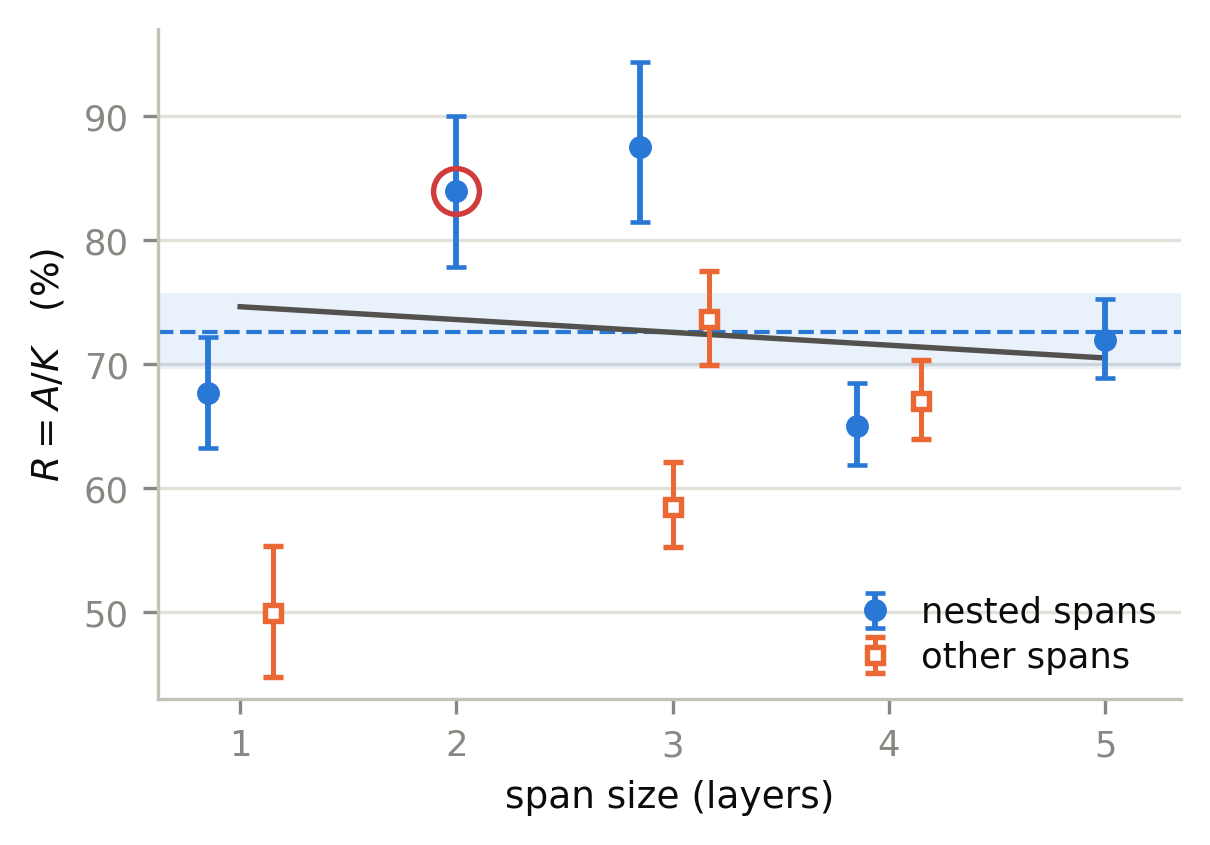
\includegraphics[width=0.66\textwidth]{fig8b_recovered_share}
  \caption{\textbf{The recovered share varies between spans but does not trend with
  span size.} $R = A/K$ with paired bootstrap intervals, the pooled value dashed and
  its interval shaded; markers as in Figure~\ref{fig:scaling}. No value lies inside
  all five nested intervals, so $R$ is not a fixed share; the fitted slope is
  $-0.010$ per layer (95\% CI $[-0.024, +0.003]$), where compensation by untouched
  layers predicts a positive slope. Plotting the other compositions at their true
  span size makes the composition effect a vertical comparison: at three layers $R$
  runs 58.5\% to 87.5\%, and at one layer 49.9\% against 67.7\%. The ringed point is
  span two, where layer 13 enters and lowers $K$ from 0.359 to 0.319, raising $R$
  without any gain in what the features recover. The trend line and pooled band
  describe the nested spans only.}
  \label{fig:rshare}
\end{figure}

\begin{table}[h]
  \centering
  \caption{Ablation at an anchor layer combined with Image$\rightarrow$Question
  knockout at all downstream layers (left), and leave-one-out marginal
  contributions to the joint five-layer ablation of 1.0028 (right).}
  \label{tab:downstream}
  \small
  \begin{tabular}{lrr@{\hskip 1.2em}lrrr}
    \toprule
    & Anchor L11 & Anchor L14 & Layer & Marginal & Standalone & Ratio \\
    \midrule
    Ablation alone            & 0.2131 & 0.2432 & 10 & $+0.1726$ & 0.1514 & 1.14 \\
    Downstream knockout alone & 0.9110 & 0.3533 & 11 & $+0.3347$ & 0.2131 & 1.57 \\
    Sum, if independent       & 1.1241 & 0.5964 & 12 & $+0.2991$ & 0.1670 & 1.79 \\
    Actual combined           & 1.2068 & 0.5989 & 13 & $+0.0862$ & 0.1220 & 0.71 \\
    Excess over additive      & $+0.0828$ & $+0.0024$ & 14 & $+0.0962$ & 0.2432 & 0.40 \\
    \bottomrule
  \end{tabular}
\end{table}

Layer 13 sits inside a band of strong cross-modal transfer and behaves unlike
its neighbours: its knockout is inhibitory at both sample sizes tested
($-0.048$ at $n = 7{,}084$, $-0.051$ at $n = 256$) while its ablation effect is
positive (0.122). The layer may host a corrective contribution to the pathway,
or the negative knockout may be an out-of-distribution effect of masking
attention at that depth; no experiment here distinguishes them. Removing layer
13 from the joint span leaves the recovered fraction at 67.0\% against 72.0\%.

% ============================================================
\bibliographystyle{plainnat}
\bibliography{refs}

\end{document}
